\section{图形的部分求和}

\subsection{骨架图形}

高阶向前散射由于泡利不相容原理其贡献为零。

\begin{figure}[htbp]
\begin{center}
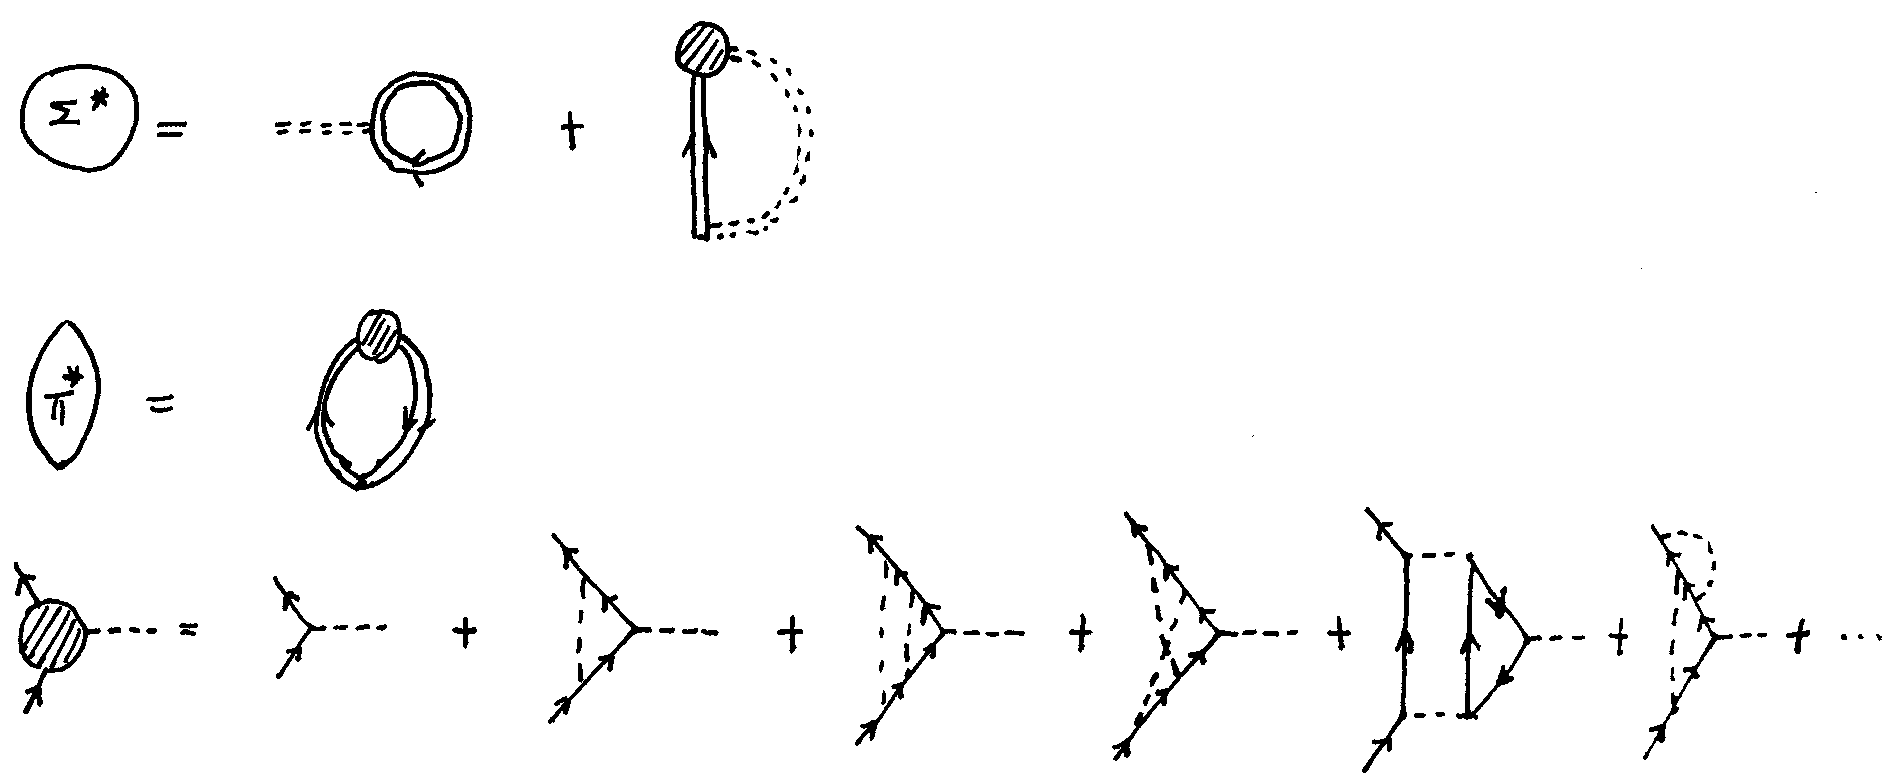
\includegraphics[width=11cm]{ManyF/skelepton.png}
%\caption{default}
%\label{default}
\end{center}
\end{figure}

正规顶角部分不能归结为有限个骨架图形的求和,这是我们无法完全精确地求出格林函数的原因。

定义双粒子格林函数:

\begin{equation}
G_2(12,34) = (-i)^2 \left\langle \Psi_H^0 \right| \mathcal{T} \{ \psi(1) \psi(2) \psi^\dagger (4) \psi^\dagger (3)  \} \left| \Psi_H^0  \right\rangle
\end{equation}

戈德斯通规定:

对于满费米球,湮灭掉一个费米球内($k < k_F $)的电子,$a_k \left| FS \right\rangle$,相对于真空态(FS)而言,能量为$- \epsilon(k)$,就是亏损了。用空穴激发(动量$-k$,能量$- \epsilon(k)$)描述多粒子系的这个态,$\epsilon^h = - \epsilon(k)$,空穴的波函数为:

\begin{equation}
\psi^h (t) = \phi(k) e^{-i (- \epsilon(k) ) t}
\end{equation}

这里可以有两种观点来看:

\begin{enumerate}
\item 

能量$\epsilon(k)$,时间$-t$,即一根逆着时间方向传播的粒子线;

\item

能量$- \epsilon(k)$,时间$t$,即一根顺着时间方向传播的粒子线;

\end{enumerate}

小结一下就是:逆着时间传播的粒子就是顺着时间传播的空穴。


%\begin{figure}[htbp]
%\begin{center}
%\includegraphics[width=15cm]{densityfluctuation.png}
%\caption{default}
%\label{default}
%\end{center}
%\end{figure}

\section{无规相近似}

\subsection{自洽的哈特利-福克近似}

只考虑自能修正($\Sigma^*$)而不考虑极化和顶角修正。

假设只计算到一阶图形:

\begin{equation}
\Sigma^*_{HF} = - 4 \pi e^2 \int_{k_1 < k_F} \frac{d^3 k_1 }{(2 \pi)^3 } \frac{1}{\left| k - k_1  \right|^2 }
\end{equation}

积分中$k$是常矢量,以$k$的方向为$z$轴建立球坐标系,$k_1$与$k$的夹角为$\theta$,

\begin{equation*}
d^3 k_1 = k_1^2 d k_1 \sin \theta d \theta d \phi
\end{equation*}

$\left|  k - k_1 \right|^2 = k^2 + k_1^2 - 2 k k_1 \cos \theta  $

\begin{eqnarray*}
\Sigma^*(k) & = & - \frac{4 \pi e^2 }{(2 \pi)^3 } \int_{k_1 < k_F} \frac{d^3 k_1}{ \left| k - k_1  \right|^2 }   \\
{}& = & - \frac{4 \pi e^2 }{(2 \pi)^3 } \int_0^{2 \pi}  \int_0^{\pi}  \int_0^{k_F} \frac{k_1^2 d k_1 \sin \theta d \theta d \phi }{ k^2 + k_1^2 - 2 k k_1 \cos \theta  } \\
{} &=& - \frac{e^2}{\pi} \int_0^{k_F} d k_1 \int_0^{\pi} \frac{k_1^2 \sin \theta d \theta }{k^2 + k_1^2 -2 k k_1 \cos \theta}
\end{eqnarray*}

变量变换:$t = \cos \theta$,$\sin \theta d \theta = - d \cos \theta$

\begin{equation*}
I = \int_0^{\pi} \frac{ k_1^2 \sin \theta d \theta  }{ k^2 + k_1^2 - 2 k k_1 \cos \theta } = \int_{-1}^{1}  \frac{k_1^2 d t }{ k^2 + k_1^2 - 2 k k_1 t  } 
\end{equation*}

变量变换:$\alpha = \frac{k }{k_1 }$

\begin{equation*}
I = \int_{-1}^1 \frac{dt}{\alpha^2 + 1 - 2 \alpha t  } = - \int_{-1}^1 \frac{d t }{2 \alpha t - (1 + \alpha^2 )  }
\end{equation*}

变量变换:$ t' = 2 \alpha t $,$d t' = 2 \alpha d t$

\begin{eqnarray*}
I &=& - \frac{1}{2 \alpha} \int_{ - 2 \alpha}^{ 2 \alpha }  \frac{ dt' }{ t' - (1 + \alpha)^2  } = - \frac{1}{2 \alpha} \left[ \ln  t'' \right]_{ - 2 \alpha - ( 1 + \alpha^2 )}^{ 2 \alpha - (1 + \alpha^2) } \\
{} & = & - \frac{1}{2 \alpha} \ln \frac{ 2 \alpha - (1 + \alpha)^2 }{ - 2 \alpha - (1 + \alpha^2 )  } = - \frac{1}{2 \alpha} \ln \frac{ \alpha^2 - 2 \alpha +1 }{ \alpha^2 + 2 \alpha +1 } \\
{} &=& - \frac{1}{\alpha} \ln \left| \frac{\alpha -1}{\alpha +1 }  \right| \\
{} &=& - \frac{k_1}{k} \ln \left| \frac{k - k_1}{ k + k_1 }  \right|
\end{eqnarray*}

现在要计算积分:

\begin{equation*}
\Sigma^*_{HF}(k ) = \frac{e^2 }{\pi}  \int_0^{k_F}  d k_1 \frac{k_1}{k} \ln \left|  \frac{ k - k_1 }{ k + k_1 } \right| 
\end{equation*}

变量变换:$ x = \frac{k_1}{ k } $, $k d x = d k_1$


\begin{equation*}
\Sigma^* = \frac{e^2 k}{\pi} \int_0^{k_F / k} x dx \ln \left| \frac{1-x}{1+x}  \right| = \frac{e^2 k}{\pi} \int_0^{k_F / k} x dx \left( \ln |1-x| - \ln |1+x|  \right)
\end{equation*}

分别考虑:

\begin{eqnarray*}
I_1 & = & \int_0^{k_F / k} x d x \ln | 1 - x |  \\
I_2 & = & \int_0^{k_F / k} x dx \ln | 1 + x |
\end{eqnarray*}

\begin{eqnarray*}
I_1 &=& \int_0^{k_F / k} \ln | 1- x | d\left( \frac{x^2}{2} \right) \\
{}&=& \left[ \frac{ x^2 \ln |1 -x| }{2} \right]_0^{k_F / k} - \int_0^{k_F / k}  \frac{x^2}{2} d \left( \ln | 1- x  | \right) \\
{} & = &  \frac{  \left( \frac{k_F}{k} \right)^2 \ln \left| 1 - \frac{ k_F }{ k } \right| }{2} - \frac{1}{2} \int_0^{k_F / k} \frac{x^2 d x}{x-1}
\end{eqnarray*}

类似地:

\begin{equation*}
I_2 = \frac{  \left( \frac{k_F}{k} \right)^2 \ln \left| 1 + \frac{ k_F }{ k } \right| }{2} - \frac{1}{2} \int_0^{k_F / k} \frac{x^2 d x}{x + 1}
\end{equation*}

\begin{equation*}
I_1 - I_2 = \frac{1}{2} \left( \frac{k_F}{k} \right)^2 \ln  \left|  \frac{ k - k_F }{ k + k_F }  \right| - \int_0^{k_F / k} \frac{x^2 }{x^2 - 1} dx
\end{equation*}

定义积分$I_3$

\begin{eqnarray*}
I_3 & = & \int_0^{k_F / k} \frac{x^2 dx}{x^2 -1} = \int_0^{k_F / k} \left( 1 + \frac{1}{x^2 - 1} \right) dx  = [x]_0^{ k_F / k  } + \frac{1}{2} \left[  \ln \left|  \frac{x-1}{x+1}   \right|  \right]_0^{k_F / k} \\
{} & = & \frac{k_F}{k } + \frac{1}{2} \ln \left| \frac{k_F - k}{k_F + k}  \right|
\end{eqnarray*}

因此:

\begin{equation*}
I_1 - I_2 = \frac{1}{2} \left(  \frac{k_F^2 - k^2}{ k^2 } \ln \left| \frac{ k-k_F }{k + k_F}  \right| \right) - \frac{k_F}{k}
\end{equation*}

代入得到HF近似下的自能:

\begin{eqnarray*}
\Sigma^*_{HF} (k) & =& \frac{e^2 k_F }{ 2 \pi } \left(  \left( \frac{k_F^2 - k^2}{ k k_F}  \right)  \ln \left| \frac{ k - k_F}{ k + k_F  } \right| - 2  \right) \\
{} & = & - \frac{e^2 k_F}{ 2 \pi } \left[ \frac{k_F^2 - k^2}{ k k_F } \ln \left| \frac{k_F + k}{ k_F - k }  \right|  + 2  \right] 
\end{eqnarray*}

\subsection*{阅读}

李正中,《固体理论》,第二版,第四章

